% !TeX root = ../cyh.tex


\chapter{内存管理模块接口的设计与实现}

\section{内存管理模块直接相关的系统调用}

\subsection{mmap 系统调用}
mmap 用于将文件或设备内存映射到进程的地址空间。它在 Linux 和类 Unix 系统中广泛使用,主要用于高效地读写文件、实现内存共享以及分配匿名内存等。

mmap 系统调用的原型如下:


\begin{lstlisting}[language=C, caption=mmap]
    void *mmap(void addr[.length], size_t length, int prot, int flags, int fd, off_t offset);
\end{lstlisting}



可以看到,mmap 系统调用共有 6 个参数,其中 addr 和 length 用于指定内存映射的起始地址和长度,prot 用于指定内存映射的保护属性,flags 用于指定内存映射的标志,fd 用于指定要映射的文件描述符,offset 用于指定文件偏移量。当 addr 为 NULL 时,表示由内核自动选择内存映射的起始地址。在 Linux 中,内核会选择一个附近的页面边界,并尝试创建映射。如果该地址已经存在另一个映射,内核会选择一个新的地址。flags 参数决定了对映射区域的更新是否对映射同一区域的其他进程可见,以及更新是否会被写入底层文件,例如,MAP\_SHARED 标志表示对映射区域的更新对所有共享该映射的进程可见,而 MAP\_PRIVATE 标志则表示对映射区域的更新对其他进程不可见。

mmap 系统调用的返回值是一个指向内存映射区域的指针,该指针指向映射区域的起始地址。如果调用失败,返回值为 MAP\_FAILED(通常为 -1)。

内存映射主要分为两种类型:匿名映射是指不与任何文件关联的内存映射,通常用于分配动态内存,类似于 malloc,但提供了更多的灵活性和控制能力,例如多个进程可以共享同一个内存映射区域;文件映射是指将文件的内容映射到内存中,这样就可以像访问内存一样访问文件的内容,通常用于实现文件的高效读写。

\begin{figure}[H]
    \centering
    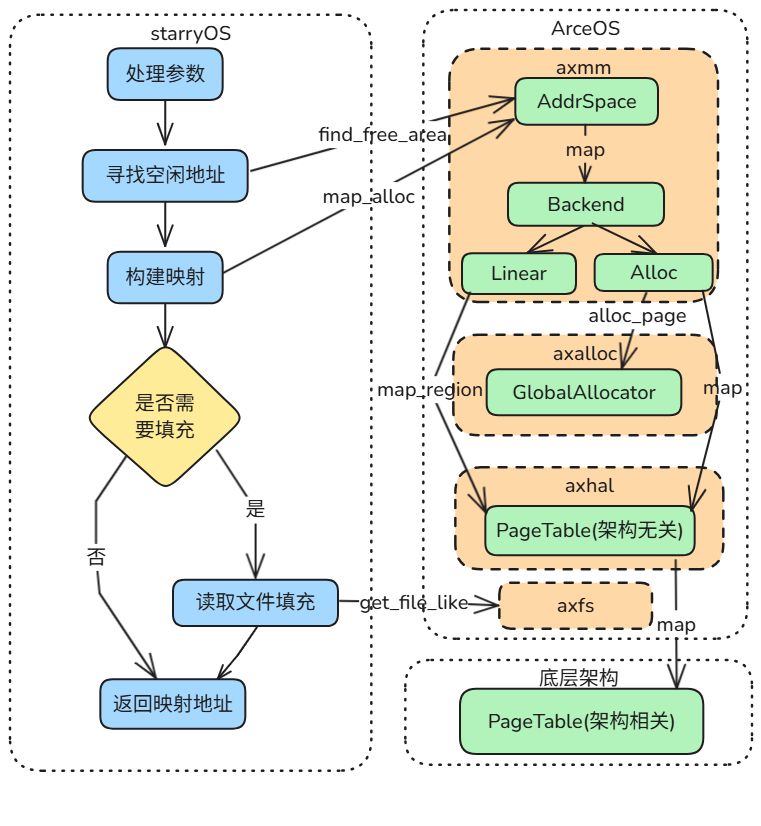
\includegraphics[width=1\linewidth, keepaspectratio]{syscall-mmap.png}
    \caption{mmap 系统调用流程}
    \label{fig:mmap}
\end{figure}

如图\ref{fig:mmap}所示,在 starry-next 中,mmap 系统调用的实现主要包括以下几个步骤:首先解析参数并检查其有效性;然后进行地址对齐处理,根据是否指定映射起始地址选择将映射长度向上对齐到 4KB (页面大小)或将映射的起始和结束地址分别对齐到页面边界;接着确定映射的真正地址:如果 flag 中设置了 MAP\_FIXED 标志,则使用对齐后的 addr 地址作为映射的起始地址,并且如果 addr 和 length 指定的内存区域与任何现有的映射重叠,那么现有映射的重叠部分将被丢弃,否则,内核会在指定地址附近或者整个用户地址空间中寻找符合条件的空闲地址,并调用 AddrSpace 结构体的 map\_alloc 方法创建映射;最后返回起始地址;如果参数中 fd 不为 -1 且 MAP\_ANONYMOUS 标志未设置,即该映射是文件映射,则在返回前需要从文件中读取数据填充到内存中。

map\_alloc 是 ArceOS 提供的一个方法,用于创建内存映射。会先验证要映射的区域,然后创建一个新的内存区域,并将其映射到页表中。
在构建映射的过程中,会根据映射的类型(线性映射或分配映射),选择不同的后端进行处理。同时还需要为映射区域分配物理页,并在页表中记录。

需要注意的是,由于 Lazy Map 机制的存在,不需要填充的内存区域不会立即被分配物理页,而是在第一次访问该内存区域并触发页面异常时才会分配物理页。该机制可能会导致内核在访问内存区域时出现 NotMapped 错误,因此需要在代码中调用 handle\_page\_fault 函数,为内存区域分配物理页,具体可以参考 AddrSpace 结构体的 clone\_or\_err 方法。

\begin{lstlisting}[language=c, caption=deal with NotMapped]
let new_addr = match new_aspace.pt.query(vaddr) {
    Ok((paddr, _, _)) => paddr,
    // If the page is not mapped, try map it.
    Err(PagingError::NotMapped) => {
        if !backend.handle_page_fault(vaddr, area.flags(), &mut new\_aspace.pt) {
            return Err(AxError::NoMemory);
        }
        match new_aspace.pt.query(vaddr) {
            Ok((paddr, _, _)) => paddr,
            Err(_) => return Err(AxError::BadAddress),
        }
    }
    Err(_) => return Err(AxError::BadAddress),
};
\end{lstlisting}


除成功返回映射的起始地址外,starry-next 中 mmap 还有其他的返回情况:MAP\_FIXED 标志设置但地址为空,或者需要从文件读取数据填充映射区域但偏移量 offset 小于 0 或者超出文件大小,函数会返回 EINVAL 错误;若系统无法找到足够的连续空闲内存区域来完成映射操作,函数会返回 ENOMEM 错误;当需要从文件读取数据填充映射区域时,若文件描述符 fd 对应的文件对象无法转换为 arceos\_posix\_api::File 类型,函数会返回 EBADF 错误。

\subsection{munmap 系统调用}

munmap 用于解除进程地址空间中的内存映射。munmap 系统调用的原型如下:
\begin{lstlisting}[language=c, caption=munmap]
int munmap(void addr[.length], size_t length);
\end{lstlisting}
munmap 系统调用共有 2 个参数,其中 addr 用于指定要解除映射的内存区域的起始地址,length 用于指定要解除映射的内存区域的长度。

munmap 系统调用的返回值是一个整数,通常为 0 表示成功,-1 表示失败。

\begin{figure}[H]
    \centering
    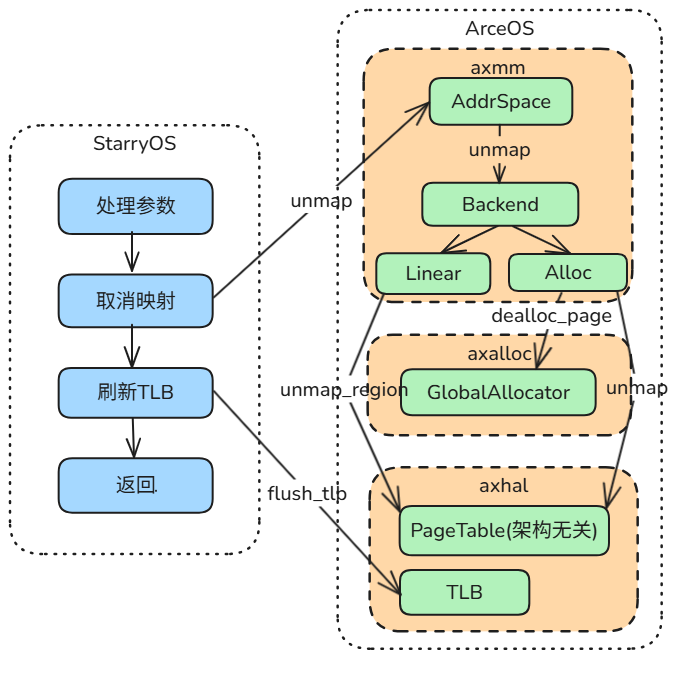
\includegraphics[width=1\linewidth, keepaspectratio]{syscall-unmap.png}
    \caption{munmap 系统调用流程}
    \label{fig:munmap}
\end{figure}

如图\ref{fig:munmap},starry-next 中,munmap 系统调用的实现主要包括以下几个步骤:首先解析参数并检查其有效性;然后调用 AddrSpace 结构体的 unmap 方法,该方法会将指定的内存区域从页表中解除映射;刷新TLB;最后返回 0 表示成功。

ArceOS 对 munmap 系统调用的支持方式与 mmap 系统调用类似,都是通过 AddrSpace 结构体向上提供接口,通过映射后端调用全局分配器和页表进行内存解除映射并释放物理页。 

另外,和 Linux 的标准实现相似,当需要取消映射的区域和当前存在的内存区域有重叠部分时,会将重叠部分的映射关系从页表中删除,并调整内存区域的起始地址和结束地址,如图\ref{fig:munmap2}所示,共存在三种情况:
\begin{enumerate}
    \item 完全覆盖:要解除映射的内存区域完全覆盖了当前存在的内存区域,此时需要将当前存在的内存区域从页表中删除,并将其从内存区域集合中移除。如图中第一项。
    \item 部分覆盖:要解除映射的内存区域位于当前存在的内存区域的中间部分,此时需要将当前存在的内存区域分为两部分,分别是要解除映射的内存区域的前半部分和后半部分,并加入到内存区域集合中,如图中第二项。
    \item 前后覆盖:要解除映射的内存区域包括当前存在的内存区域的左边界或右边界,需要调整当前存在的内存区域的起始地址或结束地址,如图中第三和第四项。
\end{enumerate}

\begin{figure}[H]
    \centering
    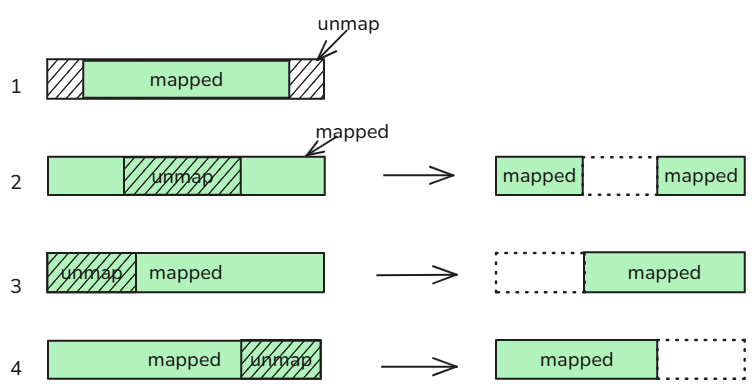
\includegraphics[width=1\linewidth, keepaspectratio]{syscall-munmap2.png}
    \caption{munmap 处理交叉区域}
    \label{fig:munmap2}
\end{figure}


\subsection{brk 系统调用}

\begin{lstlisting}[language=c, caption=brk]
int brk(void addr);
\end{lstlisting}


可以看到,brk 系统调用只有一个参数,即 addr,用于指定数据段的结束位置。
其返回值是一个整数,通常为 0 表示成功,-1 表示失败。

starry-next 中,brk 系统调用通过设置任务信息结构体的 heap\_top 字段来改变堆顶地址。具体来说,brk 系统调用会将 heap\_top 字段设置为 addr,然后返回新的堆顶,但是如果 addr 小于当前 heap\_top,或者 addr 到堆底的距离大于进程的最大数据大小限制,那么 brk 系统调用会放弃设置新的堆顶并返回原来的堆顶地址。

需要注意的是,brk 系统调用只会改变进程的堆顶位置,并不会分配实际的物理内存。因此,在使用 brk 系统调用时,需要确保进程已经分配了足够的物理内存来支持新的堆顶位置。

\begin{figure}[H]
    \centering
    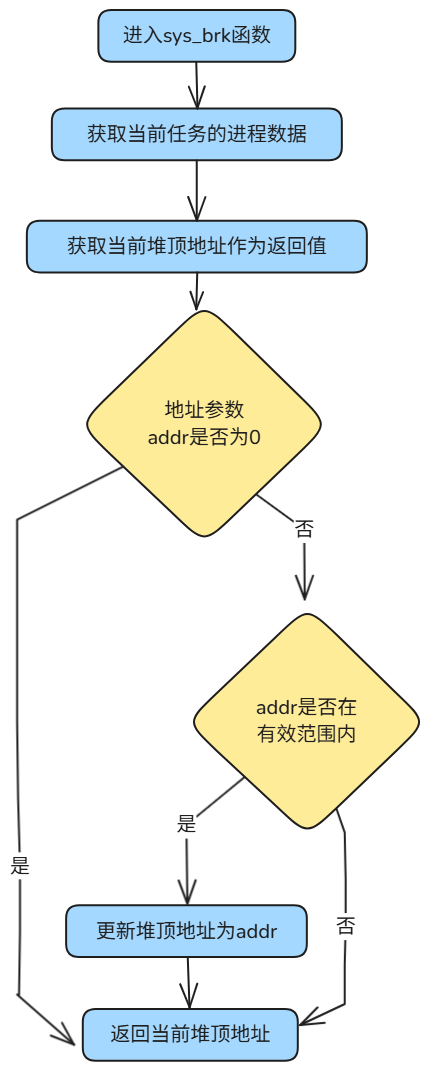
\includegraphics[width=0.5\linewidth, keepaspectratio]{syscall-brk.png}
    \caption{brk 系统调用流程}
    \label{fig:brk}
\end{figure}

\subsection{mprotect 系统调用}

mprotect 用于修改指定内存区域的保护属性。mprotect 系统调用的原型如下:
\begin{lstlisting}[language=c, caption=mprotect]
int mprotect(void addr[.len], size_t len, int prot);
\end{lstlisting}

mprotect 系统调用接受三个参数:addr(要修改权限的内存区域的起始地址,必须是页面对齐的)、len(要修改权限的内存区域的长度)以及 prot(指定新的访问权限)。prot 参数可以是PROT\_NONE(无法访问)、PROT\_READ(可读取)、PROT\_WRITE(可写入)、PROT\_EXEC(可执行)、PROT\_GROWSDOWN(向下增长)、PROT\_GROWSUP(向上增长)的按位或组合。如果进程尝试以违反保护的方式访问内存,内核将生成一个 SIGSEGV 信号。

mprotect 系统调用的返回值是一个整数,通常为 0 表示成功,-1 表示失败。可能的错误包括:EFAULT——addr 指向的地址超出了进程的地址空间、EINVAL——len 为 0 或 prot 包含无效的标志、EACCES——进程没有足够的权限来修改内存区域的保护属性、ENOMEM——内存不足等。

如图\ref{fig:mprotect}所示,在进行地址长度页对齐等参数处理后,starry-next 使用了 AddrSpace 结构体的 protect 方法,进而通过 axhal 组件的页表接口来修改内存区域的保护属性。指定范围和当前存在的内存区域的关系和处理方式与 munmap 系统调用基本一致。但暂未实现 PROT\_GROWSDOWN 和 PROT\_GROWSUP 标志的处理。

\begin{figure}[H]
    \centering
    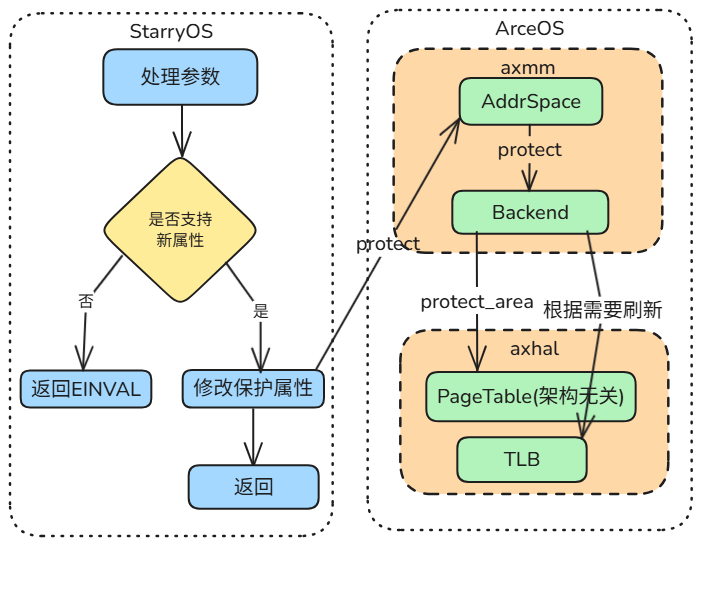
\includegraphics[width=1\linewidth, height = 8cm, keepaspectratio]{syscall-mprotect.png}
    \caption{mprotect 系统调用流程}
    \label{fig:mprotect}
\end{figure}

\section{内存管理模块间接相关的系统调用}

\subsection{sysinfo 系统调用}

sysinfo 系统调用用于获取系统的信息,如内存使用情况、CPU 信息、文件系统信息等。sysinfo 系统调用的原型如下:
\begin{lstlisting}[language=c, caption=sysinfo]
int sysinfo(struct sysinfo *info);
\end{lstlisting}
sysinfo 系统调用只有一个参数,即 info,用于存储系统信息的结构体指针。该结构体包含多个字段,例如 uptime(系统运行时间)、loads(1、5 和 15 分钟内的平均负载)、totalram 和 freeram(总内存和空闲内存)、sharedram 和 bufferram(共享内存和缓冲区内存)等。

% sysinfo 和内存管理的关系在于:sysinfo 系统调用可以获取系统的内存使用情况,包括总内存和空闲内存。因此在 ArceOS 的全局内存分配器的页分配器中,提供了接口以获取页分配器的总页数和空闲页数,这些信息可以用于计算总内存和空闲内存,并通过 sys\_sysconf 接口返回给 starry-next的 sysinfo 系统调用。

sysinfo 系统调用与包括内存管理在内的组件相关,例如通过 ArceOS 的 sys\_conf 接口获取 axconfig 组件中的核数等配置信息、axfs 组件的文件限制信息以及全局内存分配器的总页数和空闲页数;
通过 sys\_clock\_gettime 接口获取 axhal 组件的系统运行时间等。

\begin{figure}[H]
    \centering
    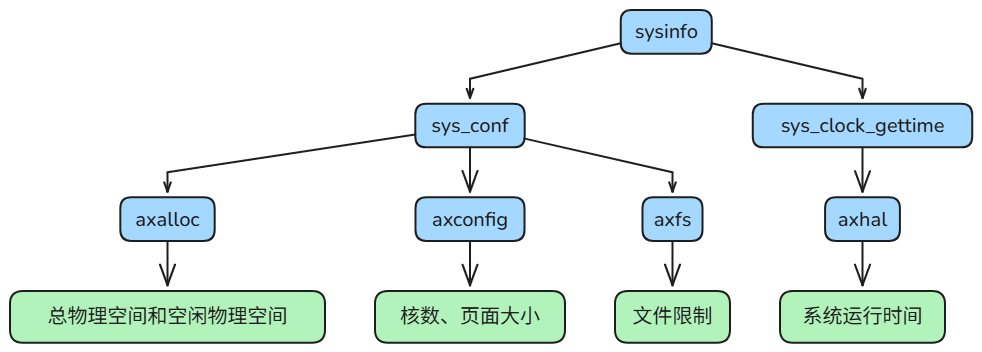
\includegraphics[width=1\linewidth, keepaspectratio]{syscall-sysinfo.png}
    \caption{sysinfo 系统调用流程}
    \label{fig:sysinfo-call}
\end{figure}

\subsection{arch\_prctl 系统调用}

arch\_prctl 系统调用用于设置或获取进程的特定架构相关的参数。其系统调用的原型如下:
\begin{lstlisting}[language=c, caption=arch\_prctl]
int syscall(SYS_arch_prctl, int op, unsigned long addr);
int syscall(SYS_arch_prctl, int op, unsigned long *addr);
\end{lstlisting}

arch\_prctl 系统调用有两个参数,code 用于指定要设置或获取的参数,addr 用于指定参数的值,设置参数时会读取 addr 指向的内容,读取参数时将结果写入其指向的地址。常见的操作包括设置或获取进程的指针追踪(Pointer Tracing)状态、设置或获取 GS 段寄存器的值等。

arch\_prctl 系统调用的返回值是一个整数,通常为 0 表示成功,-1 表示失败。

当前 starry-next 中,arch\_prctl 系统调用支持四个参数的处理:GetFs、SetFs、GetGs 和 SetGs。其中 GetFs 和 SetFs 操作用于获取和设置进程的 FS 段寄存器的值,通过读取和设置 TrapFrame(陷阱帧)中的 TLS(Thread Local Storage,线程本地存储)寄存器实现;
GetGs 和 SetGs 操作用于读取和设置进程的内核 GS 段寄存器的值,通过读取和设置 x86 架构下 msr 寄存器实现。

\begin{figure}[H]
    \centering
    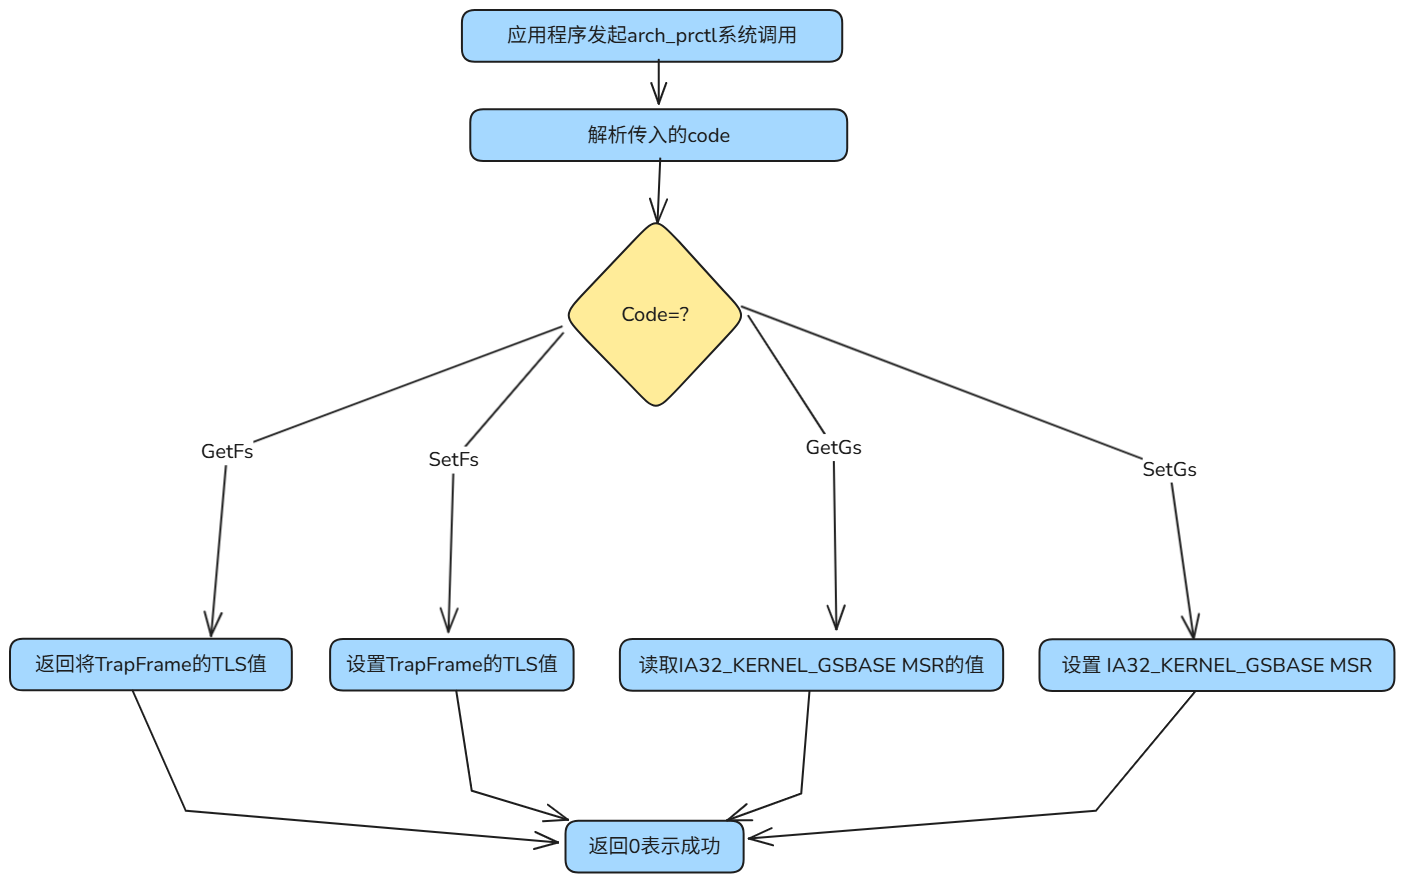
\includegraphics[width=1\linewidth, keepaspectratio]{syscall-arch-prctl.png}
    \caption{arch\_prctl 系统调用流程}
    \label{fig:arch-prctl}
\end{figure}

\subsection{prlimit64 系统调用}

prlimit64 系统调用用于设置或获取进程的资源限制,涉及操作系统的多个模块,例如栈大小和进程地址空间资源与内存管理模块有关,进程最大打开文件数与文件系统有关。prlimit64 系统调用的原型如下:
\begin{lstlisting}[language=c, caption=prlimit64]
int prlimit(pid_t pid, int resource,
            const struct rlimit *_Nullable new_limit,
            struct rlimit *_Nullable old_limit);
\end{lstlisting}

prlimit64 接受四个参数:pid——目标进程的进程ID,可以是当前进程或另一个进程)、
resource——要查询或设置的资源类型,例如 RLIMIT\_CORE(核心转储文件大小)、
RLIMIT\_CPU(CPU 时间)、RLIMIT\_DATA(数据段大小)等)、new\_limit——指向 rlimit64 结构体的指针,
用于指定新的资源限制,如果为 NULL 则表示仅获取当前限制,以及 old\_limit——指向 rlimit64 结构体的指针,
用于存储当前的资源限制,如果为 NULL 则不返回旧值。rlimit64 结构体包含 rlim\_cur(当前资源限制,又称软限制)和 rlim\_max(最大资源限制,
又称硬限制)两个字段,软限制是内核对相应资源强制执行的值,硬限制则作为软限制的上限。一个非特权进程只能将其软限制设置为从0到硬限制范围内的值,并且(不可逆地)降低其硬限制。

目前 starry-next 支持设置的资源限制包括 RLIMIT\_STACK(栈大小)和 RLIMIT\_NOFILE(最大打开文件数),二者分别通过修改进程信息结构体的 stack\_size 和 max\_files 字段来实现,其他类型的资源不会作处理。
同时限制了只有当前进程可以设置自己的资源限制,不能设置其他进程的资源限制,当传入的 pid 不为当前进程时,prlimit64 系统调用会返回 EINVAL 错误。

\begin{figure}[H]
    \centering
    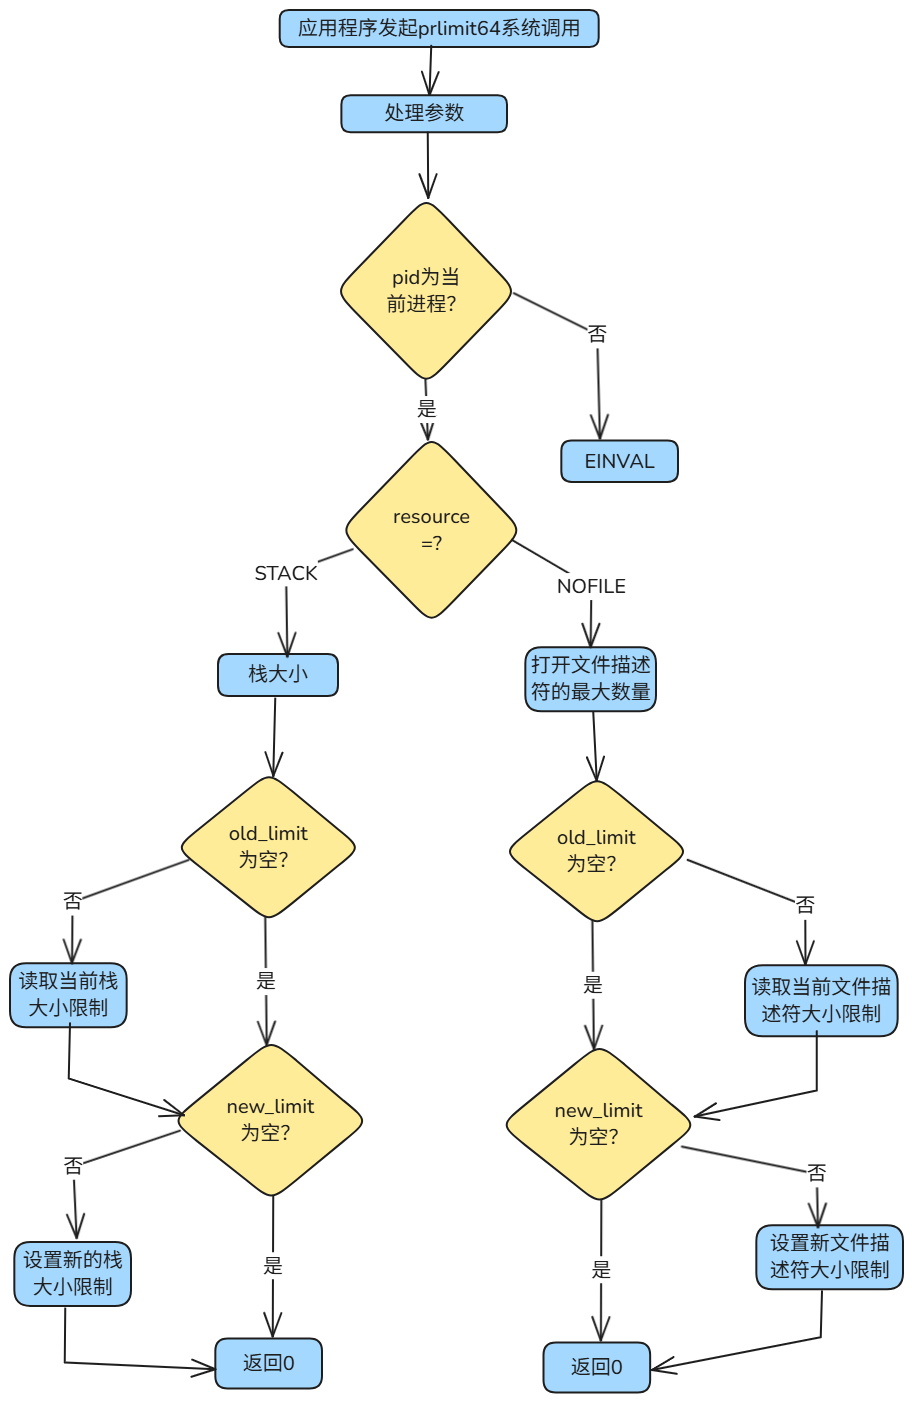
\includegraphics[width=0.5\linewidth, keepaspectratio]{syscall-prilimit64.png}
    \caption{prlimit64 系统调用流程}
    \label{fig:prlimit64}
\end{figure}
